\section{Quantum Information}


\begin{frame}
\begin{refsection}
	
\vfill

\vspace{-.5cm}\textbf{\Large Quantum Computing with \#SAT}~\cite{mei2024simulating,mei2024eq}\vspace{-.5cm}

\vfill

\printbibliography[section=\therefsection]
\end{refsection}

\end{frame}





\begin{frame}{Weighted Model Counting (\#SAT)}


Model counting (\#SAT) is the counting version ($\#\P$) of satisfiability (SAT).

\pause

~\\
~\\

\begin{definition}[Weighted Model Counting]
Given a 
	\alert{CNF formula} $F(V) \colon \mathbb B^n \to \mathbb B$ and a 
	\alert{weight function} $W\colon \set{ \bar v, v \mid v\in V} \to \mathbb{C}$, 
%For a propositional formula $F$ over variables in $V$ and weight function $W$, 
we define \concept{weighted model counting} as follows.
\[
MC_W(F) \defn   \sum_{\alpha \in  \bool^V} F(\alpha)\cdot W(\alpha)\text{, where }  W(\alpha) = \prod_{v\in V} W(\alpha(v)).
\]
\end{definition}	

\pause

\begin{example}{}
  Given the formula $F = (a \vee b) \land  c$ over $V=\{a,b, v\}$ with weights $W(a) = \frac13, W(\bar a) = \frac23$ ($a, b$ always have weight 1), the model count is:
  

\hfill 
  \begin{tabular}{|l|l|}
  \hline
  	$\bar a  b  c$ & $\nicefrac 23$ \\
  	 $a \bar b  c$ & $\nicefrac 13$ \\
  	$a b  c$ & $\nicefrac 13$\\
  \hline
  \end{tabular}  
  \hfill 
  $\nicefrac 23 + \nicefrac 13 + \nicefrac 13= \nicefrac 43$
\hfill ~

\end{example}


\end{frame}






\begin{frame}{Encoding in weighted model counting}

\vspace{-1em}
  \[
    \begin{array}{c}  
      \Qcircuit @C=1em @R=.7em {
        \lstick{\ket{0}_{\alert x}} & \qw\ar@{.}[]+<0em,1em>;[d]+<0em,-0.5em> & \gate{H ~\alert{(h)}} &\qw\ar@{.}[]+<0em,1em>;[d]+<0em,-0.5em> & \ctrl{1} & \qw\ar@{.}[]+<0em,1em>;[d]+<0em,-0.5em> &\qw & \qw\ar@{.}[]+<0em,1em>;[d]+<0em,-0.5em> &\qw & \rstick{\action<8->{\bra{0}}}  \\
        \lstick{\ket{0}_{\alert y}} & \qw & \qw & \qw & \targ & \qw &\gate{T~\alert{(t)}}&\qw &\qw& \rstick{\action<8->{\bra{0}}} \\
        & \ket{\varphi_0} & & \ket{\varphi_1} & & \ket{\varphi_2} & & \ket{\varphi_3} & &
      }
    \end{array}		
  \]

  % \begin{quantikz}
  %   \slice{\varphi_0 = \ket{0}} & \gate{H}\slice{\ket{\varphi_1}} & \ctrl{1}\slice{\ket{\varphi_2}} & \\
  %                               &                                 & \targ{}                          & \gate{T}\slice{\ket{\varphi_3}}\\
  % \end{quantikz}
 
\centering
\alert{where $x$, $y$, $h$ and $t$ are Boolean variables. We copy $x,y$ for every time step:}
 
\pause

\vspace{-1em}

\hspace{-3em}
\begin{minipage}{\textwidth}
  \begin{align*}
    \ket{\varphi_0} &&&= \ket{00} && \equiv \bar x_0 \bar y_0\\
     \action<3->{\ket{\varphi_1} &= (H \otimes I) \ket{\varphi_0} &&= \tfrac{1}{\sqrt{2}}\ket{00}+\tfrac{1}{\sqrt{2}}\ket{10} &&  
    		%F_{H_a}(\vec{x}_0, \vec{x}_1) = 
    		\equiv {\color{gray}\bar x_0 \bar y_0} ~~\land ~~ \bar y_1 h 
    							 \text{ ~~\alert{$W(h) = \nicefrac{1}{\sqrt{2}}$}} \\}
     \action<4->{\ket{\varphi_2} &= CX\ket{\varphi_1} 
    				&&= \tfrac{1}{\sqrt{2}}\ket{00}+\tfrac{1}{\sqrt{2}}\ket{11} &&
    						%F_{CX}(\vec{x}_1, \vec{x}_2) 
    						\equiv \dots  {\color{gray} h}  \dots  ~~\land ~~ (\bar x_2 \bar y_2 ~~\vee~~  x_2 y_2)\\}
     \action<5->{\ket{\varphi_3} &= (I\otimes T)\ket{\varphi_2} &&= \tfrac{1}{\sqrt{2}}\ket{00}+\tfrac{e^{i\nicefrac\pi4}}{\sqrt{2}}\ket{11} && % F_{T_1}(\vec{x}^2, \vec{x}^3) 
    			\equiv \dots  {\color{gray} h}  \dots ~~\land~~ (\bar x_3 \bar y_3 \bar t ~~\vee~~ x_3 y_3 t)}
  \end{align*}
 \pause[5]
%  $ = -\frac{1}{\sqrt{2}}$, $W(u)=e^{i\pi/4}$ and $W(\bar u)=1$.
\hfill\alert{where  $W(\bar t)=1$ and $W(t)=e^{i\nicefrac\pi4}$}
\end{minipage}

\pause

%  \keymessage{The encoding for all three gates would be
\begin{block}{Gate Encoding}
    \begin{itemize}
      \item $F_{H}(x, x',h) ~~~~~~~~\defn  \bar h \Leftrightarrow x  x' $ \hfill  
				\alert{$W(h) = \nicefrac{1}{\sqrt{2}},  W(\bar h) = -\nicefrac{1}{\sqrt{2}}$}
      \item $F_{CX}(x,y,x',y') ~~\defn   x' \Leftrightarrow  x ~~\land~~ (y'\oplus y) \Leftrightarrow  x $
      \item $F_{T}(x,x',t) ~~~~~~~~\defn x' \Leftrightarrow  x ~~\land~~  t \Leftrightarrow  x$
    \end{itemize}
\end{block}

\pause

$\bar x_0 \bar y_0 ~~\land~~  F_H(x_0,x_1, h)\alert{\land y_1 \Leftrightarrow y_0} ~~\land~~  F_{CX}(x_1,y_1,x_2,y_2)  ~~\land~~ F_{T}(y_2,y_3,t)\alert{\land x_3 \Leftrightarrow x_2} \pause ~~\land~~ \bar x_3 \bar y_3$


%  }
\end{frame}



\begin{frame}{Constructive and destructive interference}

   \[
     \begin{array}{c}  
       \Qcircuit @C=1em @R=.7em {
         \lstick{\ket{0}_x} & \qw\ar@{.}[]+<0em,1em>;[d]+<0em,-0.5em> & \gate{H} &\qw\ar@{.}[]+<0em,1em>;[d]+<0em,-0.5em> & \gate{H} & \qw\ar@{.}[]+<0em,1em>;[d]+<0em,-0.5em> &\qw \\
         & \ket{\varphi_0} & & \ket{\varphi_1} & & \ket{\varphi_2} & &
       }
     \end{array}		
   \]

  \begin{align*}
  \ket{\phi_0} &= \ket 0\\
  \ket{\phi_1} &= \frac1{\sqrt 2}(\ket 0 + \ket 1)\\
  \ket{\phi_2} &= \frac1{\sqrt 2}(\frac1{\sqrt 2}(\ket 0 \underbrace{+ \ket 1}_{}) + \frac1{\sqrt 2}(\ket 0 \underbrace{- \ket 1}_{})) &= \ket 0
  \end{align*}


\pause




~\\

\centering
$\bar x_0  ~~\land~~  F_H(x_0,x_1, h) ~~\land~~ F_{H}(x_1,x_3,h')$

\pause


~\\
~\\
Satisfying assignments at each time step:
\[
\set{\bar x_0} \quad\quad\quad\quad  \set{~ \bar x_1 h,~~  x_1h ~} 
				\quad\quad\quad\quad  \set{~ {\color{gray}\bar x_1h }\, \bar x_2 h',~~  {\color{gray} x_1h}\, \bar x_2 h',~~ {\color{gray}\bar x_1 h}\,  x_2h',~~  {\color{gray} x_1 h}\,  x_2h'  ~} 
\]

\end{frame}




\begin{frame}{Encoding in weighted model counting}
Two major problems:
\begin{itemize}
  \item Generalization of measurement is hard: e.g. measuring individual qubits will result in adding amplitudes (instead of probabilities)
  \item To check equivalence of two circuits, one has to check \alert{exponential many basis states}.
 		\[
    % \arraystretch{1.3}
  \begin{matrix*}[c]
  \text{index }\overbrace{000\dots000}^{\mathclap{\text{\alert{computational basis state}}}}:\\\text{index }{000\dots001}:\\\text{index }{000\dots010}:\\\text{index }{000\dots011}:\\\vdots\vspace{1em}\\\\\text{index }\underbrace{111\dots111}_{\vspace{3em}}:\\
  \end{matrix*}
  \left.
  \begin{bmatrix*}[c]
   i \\0 \\ 0\\ 0 \\ \vdots \\ 0 \\ 0\\ 0  \\
  \end{bmatrix*}
  \right\}\text{ $2^n$}
\]
\item Modern weighted model counter does not support \alert{complex weights}.
\end{itemize}

\pause
\vspace{2em}
{\color{red}\textbf{Solution}: Move from computational basis to Pauli basis!}

\end{frame}












\begin{frame}{Pauli basis}
        \begin{itemize}
                \item Quantum states in vector form: $\ket{\phi} = \frac{1}{\sqrt{2}}(\ket{0} + \dot{\imath} \ket{1}) 
                = \frac{1}{\sqrt{2}} \begin{bmatrix}
                        1 \\
                        \dot{\imath}
                \end{bmatrix}$
                \item Quantum states in density operator form: 
                $\dyad{\phi} = \frac{1}{2} \begin{bmatrix} 1 \\ \dot{\imath} \end{bmatrix}\cdot [1, -\dot{\imath}] = 
                \frac{1}{2}
                \begin{bmatrix}
                        1 & -\dot{\imath} \\
                        \dot{\imath} & 1
                \end{bmatrix}
                $.
        \end{itemize}

        \pause
        \[
   I\, \equiv
    \begin{bmatrix}
      1 & 0 \\
      0 & 1
    \end{bmatrix},
    \quad
    Z \equiv
    \begin{bmatrix*}[r]
      1 & 0 \\
      0 & -1
    \end{bmatrix*},
    \quad
    X \equiv
    \begin{bmatrix*}[r]
      0 & 1 \\
      1 & 0
    \end{bmatrix*},
    \quad
     Y \equiv
    \begin{bmatrix*}[r]
      0 & -\dot{\imath} \\
      \dot{\imath} & 0
    \end{bmatrix*}
.
\]
\pause

\[
        \dyad{\phi} = \frac{1}{2}(Y+I)
\]
        Note the complex numbers in the density matrix, while the Pauli coefficients are real.

\pause
\begin{block}{In general}
    Any $n$-qubit density matrix $\rho = \dyad{\phi}$  can be decomposed into in the Pauli basis:
    \[
       \rho = \sum_i \alpha_i P_i
    \]
    where $P_i\in\{I,Z,X,Y\}^{\otimes n}$ is a Pauli string and $\alpha_i\in\mathbb{R}$.
%    This result can be generalized to multi-qubit case with tensor product.
\end{block}

\end{frame}



\begin{frame}{Encoding Gates in the Pauli Basis}
	

Gates act by conjugation on density matrices / Pauli strings, e.g.: $H Z H^\dagger = X$

\pause

  \setlength{\tabcolsep}{3pt} 
  \begin{tabular}{c|rr||c|cc||c|cc}
      \toprule
      \textbf{Gate} & \textbf{In} & \textbf{Out} & \textbf{Gate} & \textbf{In} & \textbf{Out} & \textbf{Gate} & \textbf{In} & \textbf{Out} \\
      \midrule
      & $X$ & $Z$ & \multirow{6}{*}{CZ} & $\phantom{-}I_c \otimes X_t$ & $\phantom{-}Z_c\otimes X_t$ && $X$& $\frac1{\sqrt2}(X+Y)$ \\
      $H$ & $Y$ & $-Y$ & & $\phantom{-}X_c \otimes I_t$ & $\phantom{-}X_c \otimes Z_t$ & $T$ & $Y$ & $\frac1{\sqrt2}(Y - X)$ \\
      & $Z$ & $X$ & & $\phantom{-}I_c \otimes Y_t$ & $\phantom{-}Z_c \otimes Y_t$   &&$Z$ & $Z$ \\
      \cline{1-3} \cline{7-9}
       & $X$ & $Y$ & & $\phantom{-}Y_c \otimes I_t$ & $\phantom{-}Y_c \otimes Z_t$  &&$X$& $X$  \\
      $S$ & $Y$ & $-X$ & & $\phantom{-}I_c \otimes Z_t$ & $\phantom{-}I_c \otimes Z_t$  &$R_X(\theta)$& $Y$& $\cos(\theta)Y + \sin(\theta) Z$ \\
      & $Z$ & $Z$ & & $\phantom{-}Z_c \otimes I_t$ & $\phantom{-}Z_c \otimes I_t$ && $Z$& $\cos(\theta)Z - \sin(\theta) Y$\\
      \bottomrule
  \end{tabular}

\pause
\hphantom{\cite{aaronson2008improved}}




For a qubit use Boolean variables $x,z$:\\
\[
\bar x \bar z \equiv I \quad\quad\quad  x \bar z \equiv X  \quad\quad\quad x  z \equiv Y \quad\quad\quad \bar x  z \equiv Z
\]


\pause

%  \keymessage{The encoding for all three gates would be
\begin{block}{Gate encoding}
    \begin{itemize}
      \item $F_{H}(x, z, x', z', s) \defn x' \Leftrightarrow z ~\land~ z' \Leftrightarrow x ~\land~ s \Leftrightarrow xz $ \hfill  $W(s) = -1$ / $W(\bar s) = 1$
      \item \dots %$F_{CX}(x,y,x',y') ~~\defn   x' \Longleftrightarrow  x ~~\land~~ (y'\oplus y) \Longleftrightarrow  x $
\pause
      \item $F_{T}(x, z, x', z', t) \defn x' \Leftrightarrow  x ~\land~  (\bar x \Rightarrow (z' \Leftrightarrow  z)) ~\land~  t \Leftrightarrow  x \dots$ \\
		\hfill  $W(t) = \tfrac1{\sqrt 2}$ / $W(\bar t) = 1$
    \end{itemize}
\end{block}


  
	
\end{frame}



\begin{refframe}{\#SAT-based Quantum Circuit Simulation}

Simulating Quantum Circuits by Weighted Model Counting (WMC) \cite{mei2024simulating}

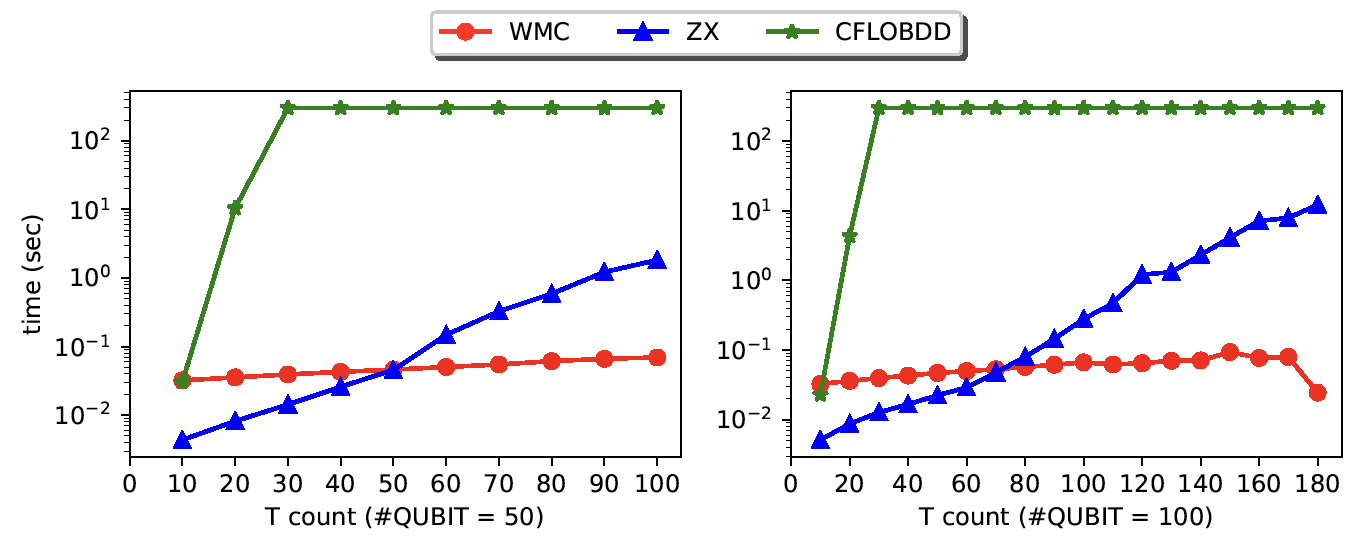
\includegraphics[height=4.5cm]{graphics/random-quokka}

Random circuits mimicking quantum chemistry applications from~\cite{kissinger_simulating_2022}.


\end{refframe}






\begin{refframe}{Encoding of equivalence checking}

\begin{definition}[Circuit Equivalence]
    Given two $n$-qubit circuits $U$ and $V$ where $n\in \mathbb{N}^+$,
    $U$ is equivalent to $V$, written $U\equiv V$, if there exists a complex number $c$ (the \concept{global phase}) such that for all input states $\ket{\psi}$, we have $U\ket{\psi} = cV\ket{\psi}$.
\end{definition}


\pause

    For an $n$-qubit quantum system, applying a single-qubit gate $P$ on the $j$-th qubit is 
 represented by 
 \begin{equation}
     P_j = I^{\otimes j -1}\otimes P \otimes I^{\otimes n- j},
     \label{eq:uj}\end{equation}

\pause

    \begin{theorem}[\cite{ours}]\label{thm:main-theorem}
        Let $U, V$ be two circuits on $n \in \mathbb{N}^{+}$ qubits.
        Then $U$ is equivalent to $V$ if and only if the following condition holds (for notation $P_j$ see \autoref{eq:uj}):\\
        For all $P \in \set{X_j, Z_j \mid j\in [n]}$, we have $U P_j U^{\dagger} = V P_j V^{\dagger}$.
    \end{theorem}

\end{refframe}


\begin{refframe}{Equivalence Checking Performance}

~
\hspace{-1.5cm}
	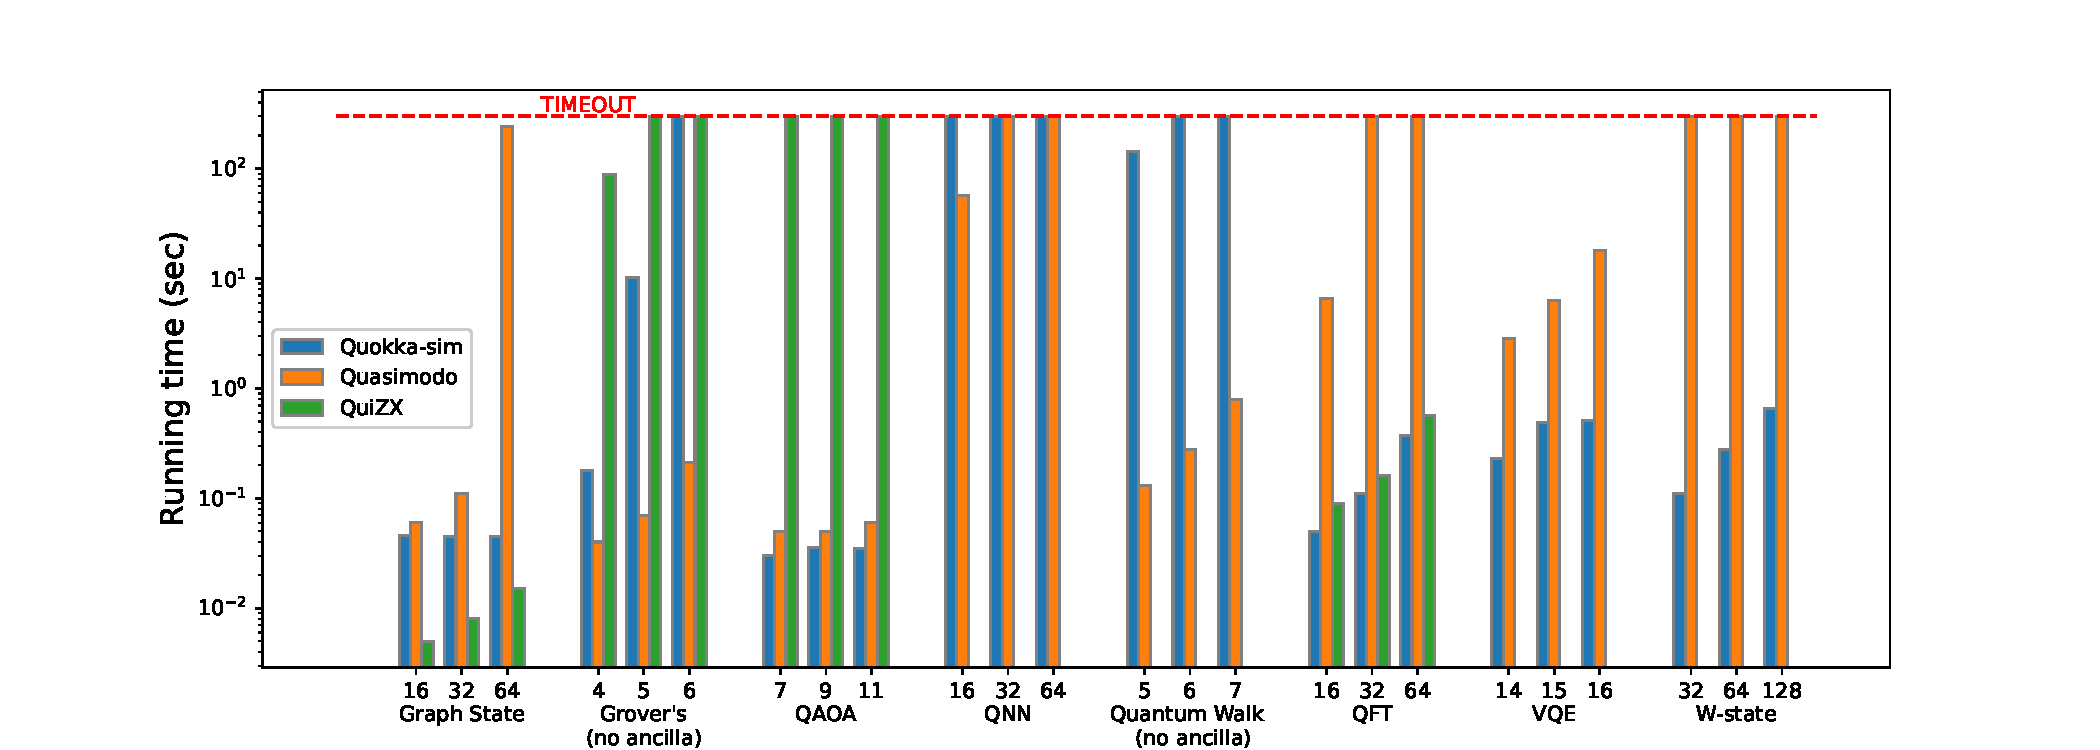
\includegraphics[width=14cm]{bar_sim}

\phantom{\cite{mei2024eq}}

\end{refframe}



\begin{refframe}{Quokka\#}

	\centering

\vspace{-4em}
	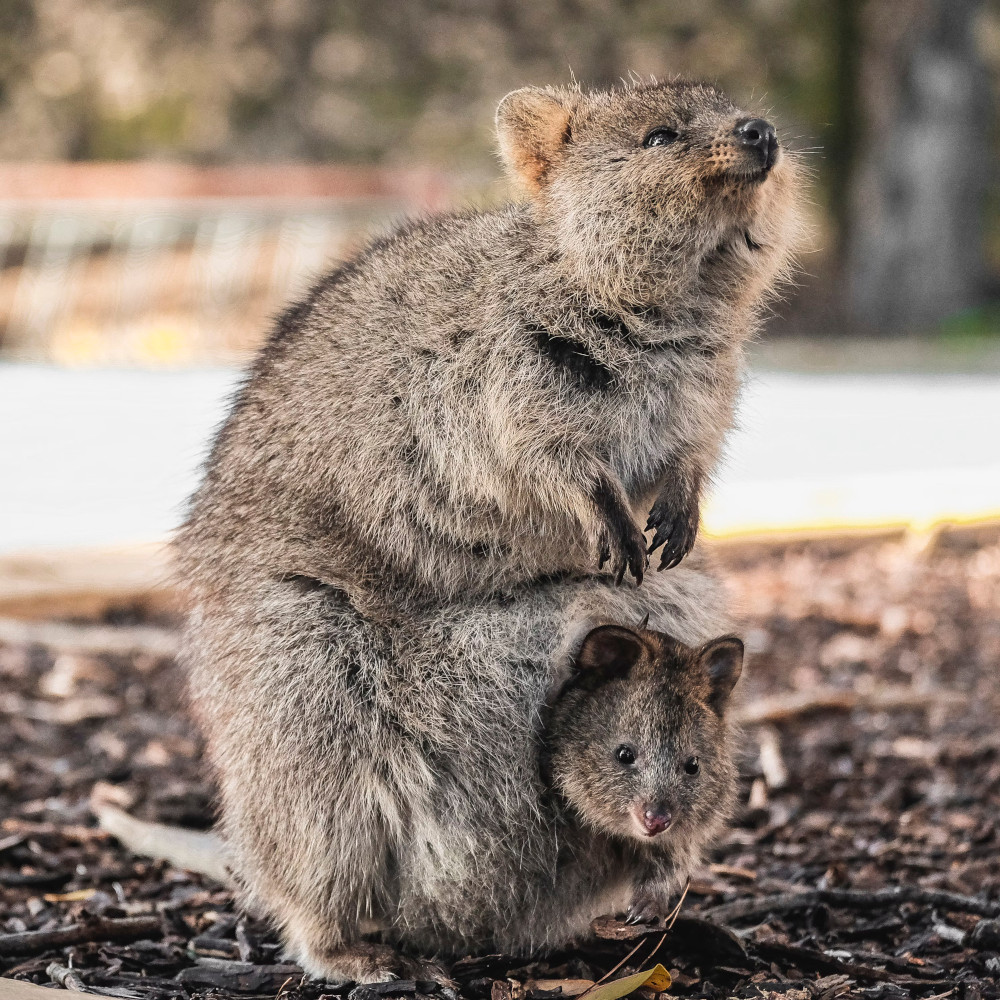
\includegraphics[width=4cm]{quokka}
	
	
\begin{alertblock}{The Quokka\# Tool}
	\begin{itemize}
		\item Linear-length \#SAT encoding of quantum circuits
		\item Simulation and equivalence checking
	\end{itemize}
	
	
\end{alertblock}

	
	\url{https://github.com/System-Verification-Lab/Quokka-Sharp}
	
	
\end{refframe}




